\documentclass[xcolor=dvipsnames,10pt]{beamer}
\usepackage[utf8]{inputenc}

\usepackage{default}
\input{/home/andi/Studium/LaTex/preambel.tex}

\definecolor{dieSchoenigste}{cmyk}{
%0,.93,.67,0.08}
.77,.71,0,0
}
\mode<presentation>{\usetheme{Ilmenau}
\usecolortheme[named=dieSchoenigste]{structure}
\setbeamercovered{transparent}}


\newcommand{\Sriro}{$\mathrm{Sr}_2\mathrm{Ir}\mathrm{O}_4$\:}
\newcommand{\Lacuo}{$\mathrm{La}_2\mathrm{Cu}\mathrm{O}_4$\:}





\title{Magnetic Excitations In The Iridate \Sriro}
\author{Andreas Leonhardt}
\institute{Det matematisk-naturvitenskapelige fakultet, UiO}
\date{13.06.2014}







\begin{document}
\begin{fmffile}{presi}
\fmfcmd{%
style_def dbl_plain_dbl_arrow expr p =
draw_double p;
shrink(1.5);
cfill (harrow (p, 0.55));
cfill (harrow (p, 0.65));
endshrink;
enddef;}


 \begin{frame}
 \titlepage
 \end{frame}


\frame{\frametitle{Contents}
 			\tableofcontents}

% MODEL FRAME, containing colums, text, items and a picture
%
% \begin{frame}
%  \frametitle{Title}
% 
%   \begin{columns} 
%     \column{.5\textwidth}
%   xxx
%   \begin{itemize}
%     \item<1-> yyy
%     \item<2-> zzz
% %   \end{itemize}
% \column{.5\textwidth}
% \includegraphics[width=\textwidth]{picture.jpg}
% \end{columns} 
% \end{frame}

\section{Iridates}

\subsection{Iridates}
\begin{frame}
 \frametitle{Motivation}
 \begin{itemize}
  \item Similar to cuprates, which are best known for HTSC
  \item Extend parameter range: enhanced SOC
  \item Spin-$\frac12$ states
  \item Realization of theoretical models: Spin models, Kitaev model,\dots
  
 \end{itemize}

\end{frame}

% what it is
% link to cuprates
% common structure


\subsection{\Sriro}

% structure: layered perovskite (maybe not that expression), effectively 2D
\begin{frame}
 \frametitle{Crystal Field}
 \begin{center}
 \includegraphics[width=.3\textwidth]{../Image_Perovskite}
 \end{center}
\end{frame}


% filling factor, SOC, relevant states
\begin{frame}
 \frametitle{Atomic States}
 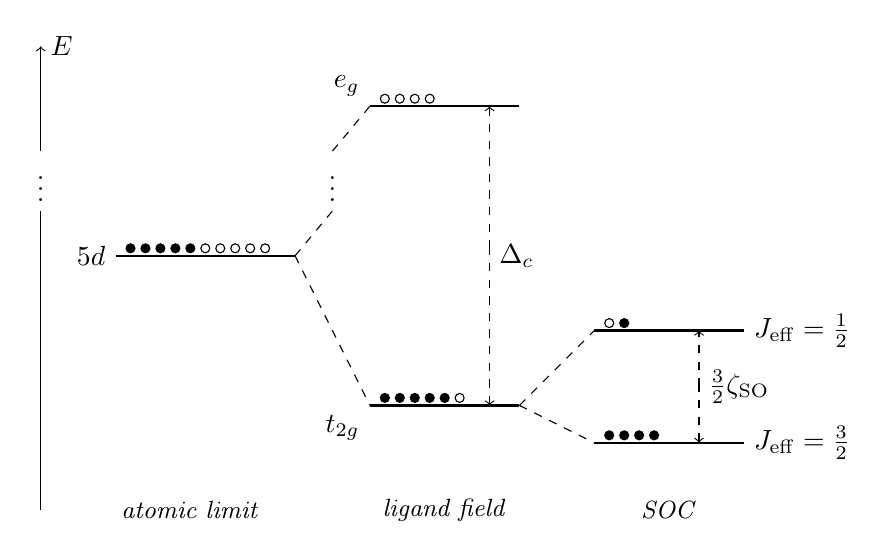
\begin{tikzpicture}[scale=1.9]
 \draw[-] (-0.7,.8) -- (-.7,2.8) node[anchor = south]{$\vdots$} ;
 \draw[->] (-0.7,3.2) -- (-.7,3.9)node[anchor =  west]{$E$};
 \draw[-,black  ,thick] (-0.2,2.5)node[anchor=east] {$5d$} -- (1.0,2.5);
 \foreach \f in {-0.1,0.0,...,0.4} \filldraw (\f,2.55) circle (0.03);
 \foreach \f in {0.4,0.5,...,0.9} \draw (\f,2.55) circle (0.03);
 %
 \draw[-,black,dashed] (1.0,2.5) -- (1.25,2.8) node[anchor= south]{$\vdots$};
 \draw[-,black,dashed] (1.25,3.2) -- (1.5,3.5);
 \draw[-,black,dashed] (1.0,2.5) -- (1.5,1.5);
 %
 \draw[-,black  ,thick] (1.5,3.5)node[anchor=south east] {$e_g$} -- (2.5,3.5);
  \foreach \f in {1.6,1.7,...,1.9} \draw (\f,3.55) circle (0.03);
 \draw[-,black  ,thick] (1.5,1.5)node[anchor=north east] {$t_{2g}$} -- (2.5,1.5);
  \foreach \f in {1.6,1.7,...,2.0} \filldraw (\f,1.55) circle (0.03);
  \draw (2.1,1.55) circle (0.03);
 %
 \draw[-,black,dashed] (2.5,1.5) -- (3,2.0);
 \draw[-,black,dashed] (2.5,1.5) -- (3,1.25);
 %
  \draw[-,black  ,thick] (3,2.0) -- (4,2.0) node[anchor= west] {$J_{\mathrm{eff}}=\frac12$} ;
  \draw (3.1,2.05) circle(0.03);
  \filldraw (3.2,2.05) circle(0.03);
 \draw[-,black  ,thick] (3,1.25) -- (4,1.25) node[anchor= west] {$J_{\mathrm{eff}}=\frac32$};
  \foreach \f in {3.1,3.2,...,3.4} \filldraw (\f,1.3) circle (0.03);
  % energie differences
  \draw[<-,black, dashed] (3.7,1.25) -- (3.7,1.625) node[anchor = west]{$\frac32\zeta_{\mathrm{SO}}$};
  \draw[->,black, dashed] (3.7,1.625) -- (3.7,2);
  %
  \draw[<-,black, dashed] (2.3,3.5) -- (2.3,2.5) node[anchor = west]{$\Delta_c$};
  \draw[<-,black, dashed] (2.3,1.5) -- (2.3,2.6);
  %
  \draw (0.3,0.8) node[]{\small{\emph{atomic limit}}};
  \draw (2.0,0.8) node[]{\small{\emph{ligand field}}};
  \draw (3.5,0.8) node[]{\small{\emph{SOC}}};
 \end{tikzpicture}
\end{frame}

\begin{frame}
 \frametitle{Unit Cell Of \Sriro}
 \begin{center}
 \includegraphics[width=.5\textwidth]{../medium.png}
 \end{center}
\end{frame}


%, AF ground state, correlated
% insulator, small ferromagnetic moment
\begin{frame}
 \frametitle{Properties Of \Sriro}
 \begin{itemize}
  \item strongly correlated
  \item insulating up to ???K
  \item small ferromagnetic moment
  \item antiferromagnetic ground state
  \item $\sum_i \langle (-1)^i n_{i,\sigma} \rangle = \sum_{\vec k} \langle c^{\dagger}_{\vec k, \sigma} c_{\vec k+\vec Q, \sigma} \rangle= \frac{s_{\sigma}}2 m_s \ne 0$
 \end{itemize}

\end{frame}


% compare to \Lacuo
% open questions: insulating type, superconducting, interactions

\section[Hubbard Model]{The Hubbard Model}

\subsection{Hubbard Model}
% give Hubbard model
\begin{frame}
\frametitle{The Hubbard Hamiltonian}
\begin{equation}
 \hat{H} = - t \sum_{\langle i,j \rangle,\sigma} \left (c^{\dagger}_{i,\sigma}c_{j,\sigma} + c^{\dagger}_{j,\sigma}c_{i,\sigma} \right) 	 
 -\mu \sum_{i,\sigma} c^{\dagger}_{i,\sigma}c_{i,\sigma} +U \sum_i n_{i,\uparrow} n_{i,\downarrow}.
\end{equation}
\end{frame}

% t term and bandstructure, relation to geometry, further interactions (i.e. t' and t'')?
% U term as simplfied interactions, how it is not first principle


% in momentum space:
\begin{frame}
\frametitle{The Hubbard Hamiltonian in momentum space}
 \begin{equation}
  \hat{H} = \sum_{\vec{k},\sigma} \left(\varepsilon_{\vec k} - \mu\right) c^{\dagger}_{\vec{k},\sigma}c_{\vec{k},\sigma} + \frac{U}{N} \sum_{\vec{k}\vec{k}^{\prime}\vec{q}}
	c^{\dagger}_{\vec{k},\uparrow}c_{\vec{k}-\vec{q},\uparrow} c^{\dagger}_{\vec{k}^{\prime},\downarrow}c_{\vec{k}^{\prime}+\vec{q},\downarrow}
 \end{equation} 
with the dispersion
\onslide<2->
\begin{equation}
 \varepsilon_{\vec k} = -2t\left( \cos k_x + \cos k_y \right) \onslide<3-> -4t^{\prime} \cos k_x \cos k_y  -2t^{\prime \prime} \left( \cos 2k_x + \cos 2k_y \right)
\end{equation}
\end{frame}

\subsection{Mean Field Equations} % or Mean Field Treatement?


% conceptual
\begin{frame}
 \frametitle{Mean Field Equations}
 \begin{itemize}
  \item<1-> neglect fluctuations
  \item<2-> each particle sees only the averaged field created by all particles
 \only<3> { \item \begin{IEEEeqnarray} {rCl}
	      U \sum_i n_{i,\uparrow} n_{i,\downarrow} &=& U \sum_i (n_{i,\uparrow}-\langle n_{i,\uparrow} \rangle ) (n_{i,\downarrow}-\langle n_{i,\downarrow} \rangle) 
	      \nonumber \\&&
	      + n_{i,\uparrow} \langle n_{i,\downarrow}\rangle + n_{i,\downarrow} \langle n_{i,\uparrow} \rangle -\langle n_{i,\uparrow} \rangle \langle n_{i,\downarrow} \rangle          
        \end{IEEEeqnarray}}
 \only<4>{  \item \begin{IEEEeqnarray} {rCl}
	      U \sum_i n_{i,\uparrow} n_{i,\downarrow} 
	      \only<4>  &\approx& U \sum_{i,\sigma} n_{i,\sigma} \langle n_{i,-\sigma}\rangle +\mathrm{const.}
        \end{IEEEeqnarray}}
        \item<5-> in momentum space: \\ $ \frac UN \sum_{\vec q} \sum_{\vec k, \vec k^{\prime}, \sigma}  c^{\dagger}_{\vec k + \vec q, \sigma} 
					    c_{\vec k, \sigma} \langle c^{\dagger}_{\vec k^{\prime} - \vec q, \sigma} c_{\vec k^{\prime}, \sigma} \rangle $
 \item<5-> uniform repulsion for $\vec q = 0$, \\ staggered magnetic field for $\vec q = \vec Q = (\pi,\pi)$. 
 \end{itemize}
 \end{frame}


\begin{frame}
\frametitle{Propagators}
 \begin{IEEEeqnarray}{rCl}
 G_{\vec k}(\tau) &=& \langle c_{\vec k         ,\sigma}(\tau)  c^{\dagger}_{\vec k ,\sigma}(0) \rangle \\
 F_{\vec k}(\tau) &=& \langle c_{\vec k +\vec{Q},\sigma}(\tau)  c^{\dagger}_{\vec k ,\sigma}(0) \rangle \label{Def_Propagator}
\end{IEEEeqnarray}
\end{frame}



\begin{frame}
 \frametitle{Mean Field Propagators}
  \begin{center}
 \begin{IEEEeqnarray}{rCl}
%\vcenter{ \hbox{
 \scalebox{.5}{\parbox{40mm}{
	      \begin{fmfgraph}(40mm,60mm)
		\fmfleft{i1}
		\fmfright{o1}
		\fmf{dbl_plain_arrow}{i1,o1}
	      \end{fmfgraph}}}
&=& \scalebox{.5}{\parbox[][][t]{30mm}{\begin{fmfgraph}(30mm,60mm) \fmfleft{i} \fmfright{o} \fmf{plain_arrow}{i,o} \end{fmfgraph}} }
   + \scalebox{.5}{\parbox{50mm}{\begin{fmfgraph}(50mm,60mm) \fmfleft{i1} \fmfright{o1} \fmf{plain_arrow}{i1,v1} \fmf{dbl_plain_dbl_arrow}{v1,o1}
					   \fmf{dashes,tension=0}{v2,v1} 	 \fmfforce{0.5w,.8h}{v2}     \fmf{dbl_plain_dbl_arrow,tension=0.7}{v2,v2}
                \end{fmfgraph}}}
	+   \scalebox{.5}{ \parbox{50mm}{\begin{fmfgraph}(50mm,60mm) \fmfleft{i1} \fmfright{o1} \fmf{plain_arrow}{i1,v1} \fmf{dbl_plain_arrow}{v1,o1}
					   \fmf{dashes,tension=0}{v2,v1} 	 \fmfforce{0.5w,.8h}{v2}     \fmf{dbl_plain_arrow,tension=0.7}{v2,v2} \end{fmfgraph}}}
 \end{IEEEeqnarray}
 \begin{IEEEeqnarray}{rCl}
 \scalebox{.5}{\parbox{40mm}{
	      \begin{fmfgraph}(40mm,60mm)
		\fmfleft{i1}
		\fmfright{o1}
		\fmf{dbl_plain_dbl_arrow}{i1,o1}
	      \end{fmfgraph}}}
&=& \scalebox{.5}{\parbox{50mm}{\begin{fmfgraph}(50mm,60mm) \fmfleft{i1} \fmfright{o1} \fmf{dbl_plain_dbl_arrow}{i1,v1} \fmf{plain_arrow}{v1,o1}
					   \fmf{dashes,tension=0}{v2,v1} 	 \fmfforce{0.5w,.8h}{v2}     \fmf{dbl_plain_arrow,tension=0.7}{v2,v2}
                \end{fmfgraph}}}
	+    \scalebox{.5}{\parbox{50mm}{\begin{fmfgraph}(50mm,60mm) \fmfleft{i1} \fmfright{o1} \fmf{plain_arrow}{i1,v1} \fmf{dbl_plain_arrow}{v1,o1}
					   \fmf{dashes,tension=0}{v2,v1} 	 \fmfforce{0.5w,.8h}{v2}     \fmf{dbl_plain_dbl_arrow,tension=0.7}{v2,v2} \end{fmfgraph}}}
\end{IEEEeqnarray} 
\end{center}
\end{frame}


% which diagrams are neglected?
% and why?

% propagators

\begin{frame}
\frametitle{Propagators}
\begin{IEEEeqnarray}{rCl}
 G_{\vec k ,\sigma}(\im \omega_n) &=& \frac{ \im \omega_n - \varepsilon_{\vec k +\vec{Q}} +\mu -Un_{-\sigma} }
					    { (\im \omega_n - E_{\vec k ,\sigma}^+) (\im \omega_n - E_{\vec k ,\sigma}^-) },
\\
 F_{\vec k ,\sigma}(\im \omega_n) &=& \frac{ Um_{s,-\sigma} }
					    { (\im \omega_n - E_{\vec k ,\sigma}^+) (\im \omega_n - E_{\vec k ,\sigma}^-)}.
\end{IEEEeqnarray}
with the poles located at
\begin{equation}
 E^{\pm}_{\vec k, \sigma} = \frac{\varepsilon_{\vec k }+\varepsilon_{\vec k +\vec{Q}}}2 -\mu + Un_{-\sigma}  \pm \sqrt{ \left(\frac{\varepsilon_{\vec k }-\varepsilon_{\vec k +\vec{Q}}}2\right)^2 + U^2m_{s,-\sigma}^2 }
\end{equation}
\end{frame}


% non-diagonal propagator and AF ground state
% staggered magnetization and $\vec Q$. 
% show staggered magnetization here
\begin{frame}
 \frametitle{Staggered magnetization}
 \begin{center}
  \includegraphics[width=.6\textwidth]{../stagmag_T10.png} \\
 Staggered magnetization as function of $\frac Ut$
 \end{center}
\end{frame}


\subsection{Dynamic Magnetic Susceptibility}

% two point correaltion function, response function
% longitudinal and transversal susceptibility
% link to scattering cross section, meaining and importance of poles
% $\omega(\vec q)$ from pole structure
% basic excitations of spin waves <--- Definition and ILLUSTRATION of SWs
\begin{frame}
 \frametitle{Excitations}
 \begin{itemize}
  \item study basic magnetic excitations by scattering experiments: neutron or X-ray (RIXS)  
  \item $\frac{\dint^2 \sigma}{\dint \omega \dint \Omega} = -2\Im \chi(\omega, \vec q) $
 \end{itemize}
\end{frame}


\begin{frame}
 \frametitle{Dynamic Magnetic Susceptibility}
 \begin{itemize}
  \item Two-point correlation function
  \item $\chi = \chi^{zz} + 2\chi^{+-}$
  \item low energy excitations only by transversal component.
 \end{itemize}

 \begin{equation}
  \chi^{+-}(\tau) = \sum_{\vec k \vec k^{\prime}} \langle c^{\dagger}_{\vec k+\vec q, \uparrow}\!(\tau)\: c_{\vec k, \downarrow}\!(\tau)\: 
		      c^{\dagger}_{\vec k^{\prime}, \downarrow}\!(0)\: c_{\vec k^{\prime}+\vec q, \uparrow}\!(0)\: \rangle
 \end{equation}
\end{frame}

% diagrammatic expansion
\begin{frame}
 \frametitle{Diagrammatic Expansion}
 \begin{IEEEeqnarray}{rCl}
  \chi^{+-} &=& 
 \scalebox{.5}{ \parbox{60pt}{ \begin{fmfgraph*}(60,50)
  \fmfleft{i1} \fmfright{o1}  \fmf{dbl_plain_arrow,left=.55}{i1,o1} \fmf{dbl_plain_arrow,left=.55}{o1,i1}
  \fmfdot{i1,o1}
 \end{fmfgraph*}}}
 \:+\: 
 \scalebox{.5}{\parbox{100pt}{  \begin{fmfgraph*}(100,50)
  \fmfleft{i1} \fmfright{o1}  \fmf{dbl_plain_arrow,left=.25}{i1,v1,o1} \fmf{dbl_plain_arrow,left=.25}{o1,v2,i1} \fmf{dashes, tension=0}{v1,v2}
  \fmfforce{.5w,h}{v1} \fmfforce{.5w,0}{v2}
    \fmfdot{i1,o1}
 \end{fmfgraph*}}} %\nonumber \\[.5cm] &&
 + \:  
 \scalebox{.5}{\parbox{180pt}{\begin{fmfgraph*}(180,50)
  \fmfleft{i1} \fmfright{o1}  
  \fmf{dbl_plain_arrow,left=0.25}{i1,v1} \fmf{dbl_plain_arrow,left=.0}{v1,v3} \fmf{dbl_plain_arrow,left=.25}{v3,o1} 
  \fmf{dbl_plain_arrow,left=.25}{o1,v4} \fmf{dbl_plain_arrow,left=.0}{v4,v2} \fmf{dbl_plain_arrow,left=.25}{v2,i1} 
  \fmf{dashes, tension=0.0}{v1,v2} \fmf{dashes, tension=.0}{v3,v4}
  \fmfforce{.33w,h}{v1} \fmfforce{.33w,0}{v2} \fmfforce{.66w,h}{v3} \fmfforce{.66w,0}{v4}
   \fmfdot{i1,o1}
\end{fmfgraph*}}}
 \:+\: \cdots
 \nonumber \\[1.5cm]
 %
 %
 \chi^{zz} &=&
 \scalebox{.5}{\parbox{40pt}{\begin{fmfgraph*}(40,50)
 \fmfleft{i1} \fmfright{o1}
 \fmf{dbl_plain_arrow,left=1.00}{i1,o1} \fmf{dbl_plain_arrow,left=1.00}{o1,i1}
 \fmfdot{i1,o1}
 \end{fmfgraph*}}}
 \:+\:
 \scalebox{.5}{ \parbox{120pt}{\begin{fmfgraph*}(120,50)
 \fmfleft{i1} \fmfright{o1}
 \fmf{dbl_plain_arrow,left=1.00}{i1,v1} \fmf{dbl_plain_arrow,left=1.00}{v1,i1}
 \fmf{dashes,tension=2.5}{v1,v2} \fmf{dbl_plain_arrow,left=1.00}{v2,o1} \fmf{dbl_plain_arrow,left=1.00}{o1,v2}
 \fmfdot{i1,o1}
\end{fmfgraph*}}}
 \:+\:
 \scalebox{.5}{ \parbox{180pt}{\begin{fmfgraph*}(180,50)
 \fmfleft{i1} \fmfright{o1}
 \fmf{dbl_plain_arrow,left=1.00}{i1,v1} \fmf{dbl_plain_arrow,left=1.00}{v1,i1}
 \fmf{dashes,tension=2.5}{v1,v2} 
 \fmf{dbl_plain_arrow,left=1.00}{v2,v3} \fmf{dbl_plain_arrow,left=1.00}{v3,v2}
 \fmf{dashes,tension=2.5}{v3,v4} 
 \fmf{dbl_plain_arrow,left=1.00}{v4,o1} \fmf{dbl_plain_arrow,left=1.00}{o1,v4}
 \fmfdot{i1,o1}
\end{fmfgraph*}}} 
\:+\: \cdots\nonumber
 \end{IEEEeqnarray}
\end{frame}





% RPA, non-crossing approximation
% geometric sum, analytical expression
% quantum corrections? mention with RPA, that a rescaling needs to be included later. 
\begin{frame}
 \frametitle{Random Phase Approximation}
 \begin{itemize}
  \item Only terms with $\vec k - \vec k^{\prime} = \vec q$ contribute
  \item No relative phase
  \item Each occurrence of $\frac UN$ is paired with a summation over $N$ momenta
  \item Closed form expression
  \item Neglecting quantum fluctuations requires rescaling 
 \end{itemize}

\end{frame}

% analytical continuation (rather not mentioning it in detail)


\section{Results}
\subsection{}
% t-U-model
\begin{frame}
 \frametitle{Results for the $t$-$U$-Model}
 \begin{center}
  \includegraphics[width=.7\textwidth]{../compare_t47} \\
 Spin wave dispersion for the $t$-$U$-model with $U=4.7t$
\end{center}
 \end{frame}
% not capable of explaining everything
% why even showing it? 
 
 
% t-t'-t''-U-model 
 \begin{frame}
 \frametitle{Results for the $t$-$t^{\prime}$-$t^{\prime \prime}$-$U$-Model}
 \begin{center}
  \includegraphics[width=.7\textwidth]{../tttU44c} \\
 Spin wave dispersion for the $t$-$t^{\prime}$-$t^{\prime \prime}$-$U$-model with $U=4.4t$
\end{center}
 \end{frame}

 
 \begin{frame}
  \frametitle{Continuous excitations}
%\begin{figure}
 \begin{center}
% \begin{subfigure}{0.49\linewidth}
  \includegraphics[width=.4\textwidth]{../fuck}
%  \caption{calculated spin wave dispersion for $U=4.4$.}
%  \label{tttU44_longw}
% \end{subfigure}
%\begin{subfigure}{.49\linewidth}
 \includegraphics[width=.4\textwidth]{../measuredexit}
% \caption{measured excitations, \\taken from \cite{PhysRevLett.108.177003} }
% \label{experimental_longw}
%\end{subfigure}
%\caption{comparison of the excitation spectrum  form our calculations and RIXS measurements. The energy scale in both graphs is given in eV. 
%	  The measured excitations contain also spin orbit excitations between 0.4eV and 0.8eV}
%\label{continuum}	  
%\end{figure}}
\end{center}
 \end{frame}
\subsection{}
 \begin{frame}
  \frametitle{Magnetization}
  \begin{itemize}
   \item $U=4.4t=1.1$eV
   \item just above the Metal insulator transition point for a SOC with $\zeta_{\mathrm{SO}} = 0.37$eV
   \item $m_s=0.73$
   \item charge gap $\Delta_{\mathrm{Mott}} = \max( E^+_{\vec k} - E^-_{\vec k^{\prime}}) =0.47\mathrm{eV}$ \\ (experimentally 0.54eV)
   % with quantum corrections: .54 = 1.18*4.6eV
  \end{itemize}
 \end{frame}
 
\begin{frame}
 \frametitle{Ferromagnetic moment}
\begin{itemize}
 \item Created by canted structure \\
 \begin{center}
   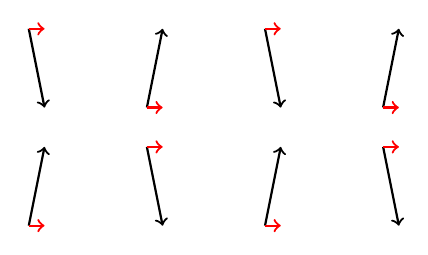
\begin{tikzpicture}
   \draw[->,thick] (-0.1,0) -- (+0.1,1);
   \draw[->,red,thick] (-0.1,0) -- (+0.1,0);
   \draw[<-,thick] (1.6,0) -- (1.4,1);
   \draw[->,red,thick] (1.4,1) -- (+1.6,1);
   \draw[->,thick] (2.9,0) -- (3.1,1);
   \draw[->,red,thick] (2.9,0) -- (3.1,0);
   \draw[<-,thick] (4.6,0) -- (4.4,1);
   \draw[->,red,thick] (4.4,1) -- (4.6,1);
  %
   \draw[<-,thick] (+0.1,1.5) -- (-0.1,2.5);
   \draw[->,red,thick] (-0.1,2.5) -- (+0.1,2.5);
   \draw[->,thick] (1.4,1.5) -- (1.6,2.5);
   \draw[->,red,thick] (1.4,1.5) -- (1.6,1.5);
   \draw[<-,thick] (3.1,1.5) -- (2.9,2.5);
   \draw[->,red,thick] (2.9,2.5) -- (3.1,2.5);
   \draw[->,thick] (4.4,1.5) -- (4.6,2.5);
   \draw[->,red,thick] (4.4,1.5) -- (4.6,1.5);
   \end{tikzpicture}
 \end{center}
 \item $\frac{M}{M_{\mathrm{local}}} = m_s \sin \Theta = 0.139$
 \item experimentally $M = 1.14\mu_b$ 
 \item $M_{\mathrm{local}} = 1\frac{\mu_b}{\mathrm{Ir}^{4+}}$, as in the  atomic limit
\end{itemize}
\end{frame}


 
 
 
% limiting case, comparison to Heisenberg and linear spin waves
% t-t'-t''-U-Hubbard model results
% t-U-Hubbard model?
% point out the meaning of the result. 

%implications
% U=4.4 =1.1eV
% insulator type?

\subsection{Further Prospects/ Outlook}

% improvements
\begin{frame}
 \frametitle{Improvements}
 \begin{itemize}
  \item Quantum corrections
  \item Refine Band structure
 \end{itemize}
\end{frame}

 \begin{frame}
 \frametitle{Further Calculations}
 \begin{itemize}
  \item Change filling factor
  \item Different materials
 \end{itemize}

\end{frame}

% corrections
% other materials, other filling factors.

\section*{}
\begin{frame}
 \frametitle{}
 \begin{center}
  Thank you for your attention.
 \end{center}

\end{frame}


\end{fmffile}

\end{document}
